\section{Literaturrecherche} \label{stand-der-technik-literaturrecherche}

Um einen Überblick über den aktuellen Stand der Forschung zu bekommen wird zunächst eine Literaturrecherche vorgenommen. Dabei sollen vorhandene online IDEs gefunden sowie die folgenden Fragen beantwortet werden:

\begin{itemize}
    \item Welche Implementierungen von online IDEs gibt es?
    \item Welchen Architekturmustern folgen online IDEs?
    \item Welche Vor- und Nachteile haben die online IDEs?
    \item Welche Anforderungen werden an online IDEs gestellt?
\end{itemize}

Die folgenden Datenbanken wurden für die Literaturrecherche ausgewählt:

\begin{itemize}
    \item ACM Digital Library
    \item IEEE Xplore
    \item Scopus
    \item Web of Science
\end{itemize}

Zunächst wurde eine allgemeine Suche nach online IDEs in den genannten Datenbanken vorgenommen. Dazu werden zunächst die in Tabelle \ref{table:search-terms} genannten Stichwörter jeweils mit ihren Synonymen mit einer OR-Operation verknüpft. Danach werden die daraus resultierenden Terme mit einer AND-Operation verbunden. Die so entstehende Suchanfrage werden dann für die Suche in den Datenbanken verwendet. Dabei werden die Titel, Abstracts und Keywords der Publikationen durchsucht.

In Tabelle \ref{table:amount-search-results} ist die Anzahl der Treffer für den einzelnen Datenbanken dargelegt. Um die Anzahl der zu betrachtenden Publikationen zu verringern wird eine weitere Filterung der Ergebnisse vorgenommen. Dafür werden nur Publikationen betrachtet, die IDE oder ein entsprechendes Synonym in ihrem Titel oder ihren Keywords enthalten. Dadurch sinkt die Anzahl der Treffer auf insgesamt $1705$. Danach werden alle exakten Duplikate über einen Vergleich der Titel und Links herausgefiltert wodurch die Anzahl der Publikationen auf $1243$ sinkt. In einem weiteren Schritt werden die Titel und Abstracts der Publikationen genauer betrachtet. Dabei werden unter anderem Arbeiten herausgefiltert, deren Titel und Abstracts keinen Bezug zu den Forschungsfragen besitzen. Weiterhin werden Publikationen bevorzugt, die sich zudem mit textbasierten Programmiersprachen, Kollaboration und Lehre auf Universitätsniveau befassen. Aus dieser Filterung resultieren $97$ Publikationen. Als letzte Filterung werden Publikationen, welche vor $2019$ veröffentlicht wurden aussortiert, falls sie weniger als $10$ Zitationen haben sowie vor $2014$ veröffentlichte Publikationen mit weniger als $25$ Zitationen. Die Anzahl der Zitationen wurde mithilfe von Google Scholar ermittelt. Dadurch ergibt sich die Anzahl von $64$ zu betrachtenden Publikationen.

\begin{table}[tbp]
    \centering
    \begin{tabularx}{\textwidth}{| >{\hsize=.6\hsize\linewidth=\hsize}X |
            >{\hsize=1.4\hsize\linewidth=\hsize}X |}
        \hline
        Stichwort                           & Synonyme                                                                                                     \\
        \hline
        integrated development environments & IDEs, code editors, development environments, development tools, programming tools, programming environments \\
        \hline
        web                                 & browser, online, cloud                                                                                       \\
        \hline
    \end{tabularx}
    \caption{Suchbegriffe}
    \label{table:search-terms}
\end{table}

\begin{table}[tbp]
    \centering
    \begin{tabular}{|c|c|c|c|c|c|}
        \hline
        ACM & IEEE & Scopus & Web of Science \\
        \hline
        785 & 1472 & 4661   & 1044           \\
        \hline
    \end{tabular}
    \caption{Anzahl Suchergebnisse}
    \label{table:amount-search-results}
\end{table}

\begin{figure}[htbp]
    \centering
    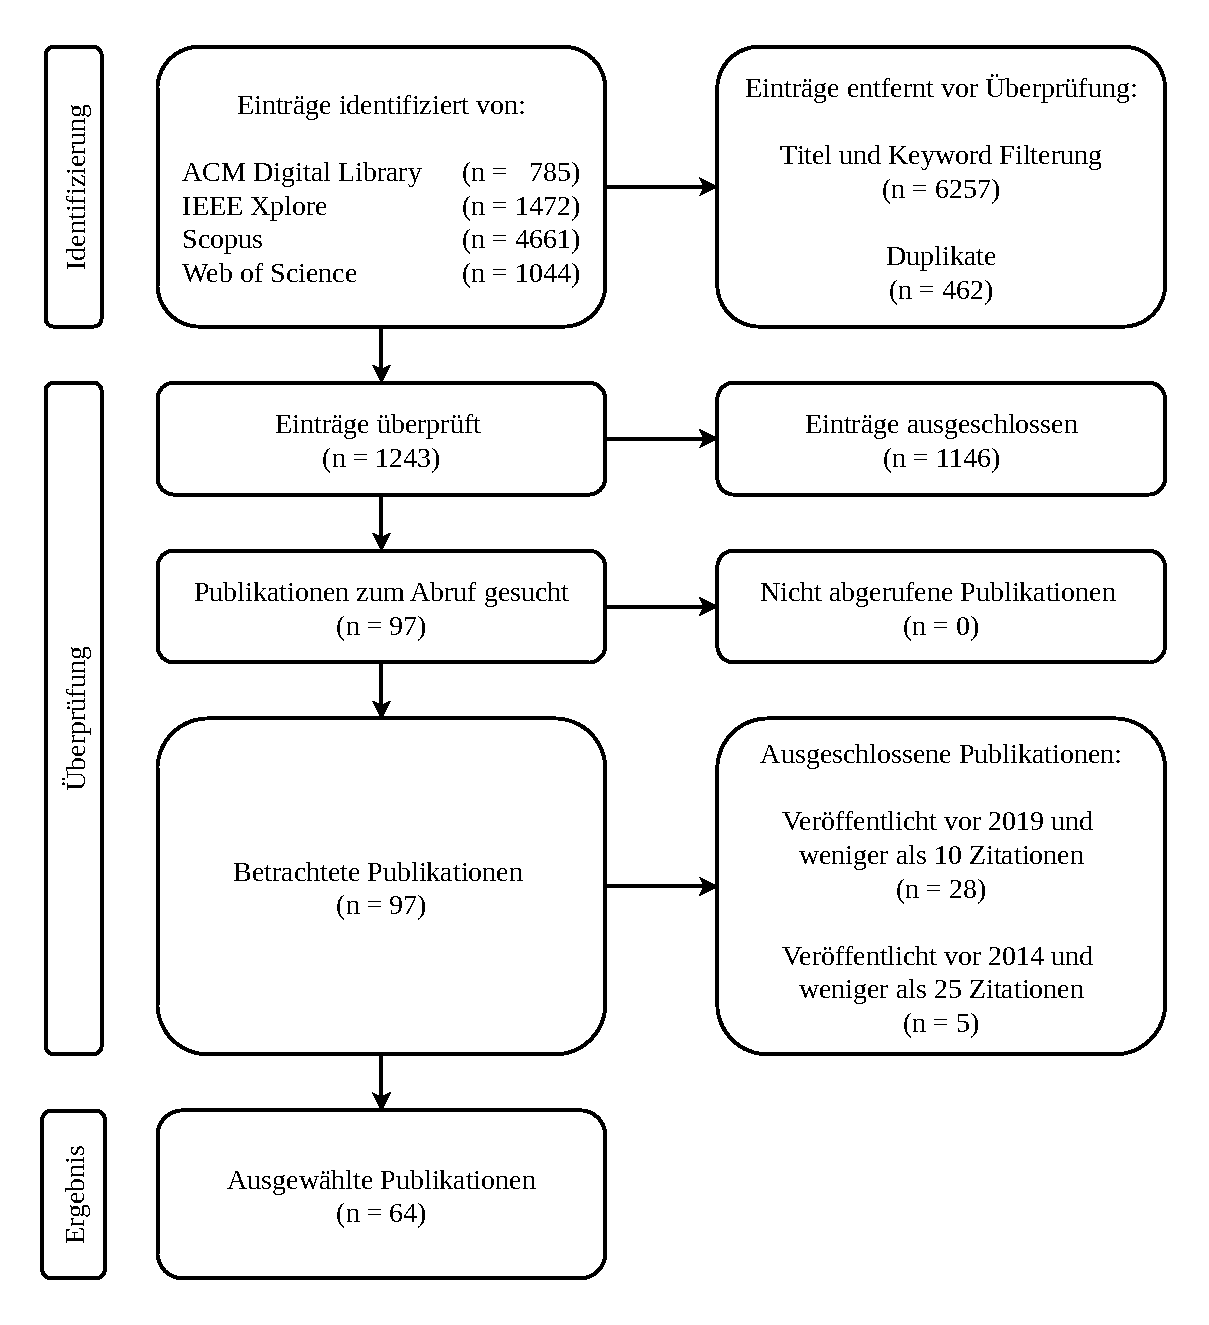
\includegraphics[width=\textwidth]{diagrams/PRISMA.pdf}
    \caption{PRISMA Diagramm}
    \label{prisma-diagram}
\end{figure}

Die Publikationen beschreiben eine Vielzahl an verschiedenen webbasierten integrierten Entwicklungsumgebungen. Dabei kann eine Unterteilung in die folgenden zwei Kategorien erfolgen:

\begin{itemize}
    \item \textbf{Client-Server-basierte Lösungen} \\
          Systeme dieser Art zeichnen sich dadurch aus, dass sie eine Client-Server-Archi-tektur verwenden. Hierbei werden Features, die nicht innerhalb eines Browsers ausgeführt werden können (z.B. Kompilierung) über einen entsprechenden Server bereitgestellt.
    \item \textbf{Browser-basierte Lösungen} \\
          Systeme dieser Art zeichnen sich dadurch aus, dass alle Features im Browser des Nutzers ausgeführt werden können, ohne die Hilfe eines separaten Servers.
\end{itemize}

Deursen et al. (2010) \cite{van_deursen_adinda_2010} beschreiben eine online IDE names Adinda. Die grundlegende Idee von Adinda ist die Zerlegung der Funktionalität einer IDE in einen leichtgewichtigen Client sowie mehrere zusammenarbeitende (Web-)Services. Diese Services sollen dann bestimmte Aufgaben erfüllen, wie z.B. Kompilierung, Testen, kollaboratives Editieren und Datenerhebung. Es werden weiterhin verschiedenste Forschungsfragen aufgestellt, die für das vorgestellte System von Interesse sind. Die prototypische Implementierung von Adinda basiert auf WWWorkspace \cite{ryan_web_2007} und nutzt serverseitig Eclipse \cite{noauthor_eclipse_nodate}. Der Prototyp unterstützt das Erstellen von Nutzer-Workspaces, Java Projekten, Paketen und Klassendateien sowie Syntax Highlighting, Kompilierung und Code-Vervollständigung. \todo{Adinda}

Wu et al. (2011) \cite{wu_ceclipse_2011} stellen die online IDE Cloud Eclipse (CEclipse) vor. Die Ziele von CEclipse sind:
\begin{enumerate}
    \item die Bereitstellung von Eclipse \cite{noauthor_eclipse_nodate} Funktionen wie z.B. Code-Vervollständigung
    \item die Behandlung von den online IDE spezifischen Sicherheitsproblemen \quoted{\textit{Wrong file operations}}, \quoted{\textit{Banned operation calling}} und \quoted{\textit{Excessive resource consumption}}
    \item die Ausnutzung von Cloud Computing Möglichkeiten um Entwickler besser zu unterstützen.
\end{enumerate}
Für $1.$ wurde ein entsprechendes Protokoll entwickelt, was es ermöglicht die gewünschten Funktionen von Eclipse aufzurufen und das Ergebnis im Browser darzustellen. Um die in $2.$ genannten Probleme Handhaben zu können wird ein \textit{Program Behavior Analysis Service} beschrieben. Durch die Einschränkung des Dateisystems auf einen speziellen Ordner kann das Problem \quoted{Wrong file operations} gelöst werden. Das Verbieten bzw. Erlauben von Methoden über eine Blacklist bzw. eine Whitelist kann zur Lösung des Problems \quoted{Banned operation calling} angewendet werden. Durch eine Zeitbegrenzung von laufenden Prozessen kann schließlich auch das Problem \quoted{Excessive resource consumption} behoben werden. Für $3.$ werden über den \textit{Program Behavior Mining Service} Daten über die Nutzung der IDE gesammelt werden. Diese Daten können dann z.B. dazu genutzt werden dem Entwickler häufig verwendete Befehle mit höherer Priorität vorzuschlagen. \todo{CEclipse}

Goldman et al. (2011) \cite{goldman_real-time_2011} beschreiben Collabode, eine kollaborative online IDE für Java. Collabode ermöglicht es mehreren Nutzern gleichzeitig Änderungen an Dateien vorzunehmen. Die Änderungen werden in Echtzeit zwischen den Nutzern synchronisiert. Dabei wird ein spezieller Algorithmus verwendet. Dieser Algorithmus sorgt dafür, dass nur Änderungen eingepflegt werden, die keinen syntaktischen Fehler beinhalten oder erzeugen. Dadurch wird sichergestellt, das Nutzer nur ihre eigenen Fehler sehen und das Programm unabhängig von den ggf. vorhandenen Fehlern ihrer Teammitglieder kompilieren können. Collabode nutzt EtherPad \cite{noauthor_etherpad_nodate} als Editor im Frontend und Eclipse \cite{noauthor_eclipse_nodate} für die Bereitstellung von Kompilierung, Syntax Highlighting, etc. im Backend. \todo{Collabode}

Lautamäki et al. (2012) \cite{lautamaki_cored_2012} stellen Collaborative Real-time Editor (CoRED) vor, einen online Code Editor für Java Programme. CoRED nutzt den ACE Editor \cite{noauthor_ace_nodate} im Fronted sowie das Java Development Kit (JDK) \todoaddref[]{JDK} zur Kompilierung im Backend. Fehlermeldungen während des Kompiliervorgangs werden an den Client zurückgesendet und dann im Frontend visualisiert. Zur Bereitstellung von Echtzeit Kollaboration wird der Algorithmus \textit{Differential Synchronization with shadows} \cite{fraser_differential_2009} von Neil Fraser eingesetzt. Ein weiteres Feature von CoRED ist das Sperren von Code Bereichen für andere Nutzer sowie die Möglichkeit Kommentare im Code zu hinterlassen. Auf diese Kommentare können dann andere Nutzer antworten, wodurch eine weitere Interaktionsmöglichkeit besteht. Weiterhin bietet CoRED auch Code-Vervollständigung an. \todo{CoRED}

Tran et al. (2013) \cite{tran_interactive_2013} stellt die online IDE IDEOL vor. IDEOL erlaubt es Nutzern in Echtzeit miteinander zu kollaborieren. Dies beinhaltet das gleichzeitige Bearbeiten von Dateien mit Synchronisierung der Änderungen zwischen den Nutzern sowie ein Diskussionsforum mit einem Tagging-Mechanismus. Über diesen Mechanismus können Nutzer Codezeilen oder ganze Dateien in einer Diskussion taggen. Weiterhin können Nutzer auch Dateien an ihre Nachrichten anhängen. Zudem bietet IDEOL eine Übersicht über die Änderungen im Code. IDEOL bietet Support für die Entwicklung von C/C++ Programmen und erlaubt auch die Kompilierung, Ausführung sowie das Debugging von diesen. Um die Echtzeit Kollaboration zu ermöglichen unterscheidet IDEOL zwischen exklusiven und nicht-exklusiven Operationen. Zu den exklusiven Operationen zählen die Kompilierung, Ausführung und das Debugging eines Programms. Dateien werden über einen Server synchronisiert und dort gespeichert. Die Behandlung von gleichzeitigen Operationen wird mithilfe eines Operational Transformation Algorithmus \todoaddref[]{Operational Transformation IDEOL} vorgenommen. Exklusive Operationen werden auf der im Server persistent gespeicherten Version ausgeführt, sodass die im Arbeitsspeicher des Servers vorhandene Version weiterhin zur Bearbeitung verwendet werden kann. \dots \\
Nguyen et al. (2016) \cite{nguyen_enhancing_2016} \dots \todo{IDEOL/EduCo}

Ball et al. (2015) \cite{ball_beyond_2015} beschreiben TouchDevelop. TouchDevelop ist eine online IDE bzw. eine cloudbasierte IDE (CIDE). Das Hauptfeature von TouchDevelop ist die Speicherung aller Programmänderungen, Versionen, Laufzeitinformationen, Bugs sowie Kommentare, Fragen und Feedback von Nutzern in einer zentralen Datenbank. Diese Daten können über entsprechende APIs abgefragt werden. Die Nutzeroberfläche von TouchDevelop unterscheidet sich stark von anderen textbasierten Editoren. So bekommt der Nutzer eine Auswahl an kontextabhängigen Optionen, z.B. if-Anweisungen, for-Schleifen oder verfügbare Variablen. Alle IDE Funktionen sind offline verfügbar, da sie komplett auf der Clientseite implementiert sind. Weiterhin nutzt TouchDevelop eine eigene Programmiersprache. Diese folgt dem imperativen Programmierparadigma, besitzt ein starkes Typsystem sowie eine Vielzahl an plattformübergreifenden APIs. \dots \todo{TouchDevelop}

Warner und Guo (2017) \cite{warner_codepilot_2017} stellen die online IDE CodePilot vor. Diese ermöglicht es Nutzern Webapplikationen mithilfe von HTML, CSS und JavaScript zu entwickeln. Zudem können Nutzer mithilfe von Firepad \todoaddref[]{Firepad} gleichzeitig an Projekten arbeiten. Weiterhin bietet CodePilot eine GitHub \todoaddref[]{GitHub} Integration, wodurch Nutzer ihre Projekte aus GitHub importieren können. Über diese Integration werden auch bei jedem Commit die entsprechenden Änderungen an GitHub zurückgesendet. Weiterhin können Nutzer über einen Aktivitätsfeed die aktuellen Ereignisse nachverfolgen und mithilfe eines integrierten Text-Chats miteinander kommunizieren. Weiterhin werden durch den Ace-Editor \cite{noauthor_ace_nodate} Syntax Highlighting und Code-Vervollständigung bereitgestellt. Zusätzlich bietet CodePilot die Möglichkeit Issues zu erstellen. Diese werden dann mit GitHub synchronisiert und es wird ein Snapshot des aktuellen Projekts auf GitHub hinterlegt. Bei der Erstellung einer Issue können auch Screenshots angefügt werden. Jede Issue enthält die Referenz auf den entsprechenden Snapshot des Projekts. \dots \todo{CodePilot}

Über mehrere Publikationen wird die Entwicklung der Reflex IDE (RIDE) beschrieben.  Zunächst wird von Bastrykina et al. (2021) \cite{bastrykina_developing_2021} ein entsprechender Kernel mit dem Xtext Framework \cite{noauthor_xtext_nodate} entwickelt, welcher in der Eclipse IDE verwendet werden kann, um diese \todo{}. Darauf aufbauend wird von Gornev und Liakh (2021) \cite{gornev_ride_2021} die Konzipierung und Implementierung einer auf Theia basierten Web-Variante von RIDE vorgestellt. Gornev et al. (2022) \cite{gornev_towards_2022} beschreiben ein System, welches Docker verwendet um die Web-Version von RIDE für mehrere simultane Nutzer bereitstellen zu können. Gornev und Bondarchuk (2023) \cite{gornev_towards_2023} entwickeln ein Framework, welches es erlaubt Echtzeit-Kollaboration in Single-User Anwendungen zu ermöglichen. Kuznetsov und Zyubin (2024) \cite{kuznetsov_development_2024} beschreiben die Entwicklung eines Projektmanagement-Systems für RIDE. \todo{RIDE}

Jefferson et al. (2024) \cite{jefferson_pyodideu_2024} beschreiben eine IDE, die es Nutzern ermöglicht Python Code im Browser zu schreiben und auszuführen. Dabei wird das Programm des Nutzers lokal in dessem Browser durchgeführt. Dies wird durch den Einsatz von PyodideU erreicht, einer erweiterten Version der WebAssembly-basierten Python Distribution Pyodide \cite{noauthor_pyodide_nodate}. Zusätzlich wird den Nutzern auch eine Grafikbibliothek angeboten samt eines Debuggers, der es ermöglicht Zeile für Zeile und auch rückwärts durch das Programm zu gehen und die entsprechenden Änderungen an der Grafik zu sehen. Weiterhin wird durch PyodideU auch die synchrone Eingabe von Daten unterstützt, während Python im Main-Thread des Browsers läuft. Zudem wird auch ein Dateisystem bereitgestellt. Insgesamt wurde die IDE sowohl von Studenten als auch von Lehrenden als hilfreich wahrgenommen. \todo{PyodideU}

Malan (2024) \cite{malan_containerizing_2024} beschreibt die verschiedenen Ansätze zur Bereitstellung einer integrierten Entwicklungsumgebung für die Teilnehmer des Einführungskurses in die Programmierung (CS50) an der Harvard University. Zunächst wurde seit 2007 ein On-Campus Cluster für die Studenten angeboten. Studenten konnten über SSH mit diesem verbinden und dort ihre Programme ausführen. Dieser Cluster wurde 2008 mithilfe von Amazon Web Services (AWS) \cite{noauthor_amazon_nodate} in die Cloud überführt. Diese cloud-basierte Lösung wurde 2011 durch Client-seitige virtuelle Maschinen ersetzt. In 2015 wurde eine auf Docker basierende Lösung erarbeitet, die zunächst Cloud9 IDE \cite{noauthor_cloud_nodate} als Frontend nutzte. In 2021 wurde schließlich eine auf Github Codespaces aufbauende Lösung eingeführt, die Visual Studio Code (VSCode) \todoaddref[]{VSCode} als Code Editor verwendet. \todo{CS50}

% Vorteile:
% \begin{itemize}
%     \item + Keine Installation
%     \item + Keine Zeitrestriktion (im Gegensatz zu Computerlaboren)
%     \item + Vorbereitete Entwicklungsumgebung mit allen benötigten Tools und Bibliotheken bereits vorgegeben
%     \item + Gleiche Entwicklungsumgebung für alle
%     \item + Einfacheres Teilen von Projekten
%     \item + Vereinfachte Kollaboration
%     \item + Von überall nutzbar
%     \item + Gleiche Daten auf allen Geräten (bei Server-Speicherung)
%     \item + Ggf. kein leistungsstarker Rechner notwendig
%     \item + Skalierbarkeit
%     \item + Einbindbarkeit in LMS
%     \item + Offline Nutzbarkeit von browserbasierten IDEs
%     \item + Einfachere Datenerhebung
%     \item (Einfaches Nutzerinterface)
% \end{itemize}

Der am meisten genannte Vorteil von online IDEs ist die Tatsache, dass diese keine Installation benötigen. Somit wird es Nutzern ermöglicht direkt mit der Programmierung zu beginnen ohne zuvor die benötigte Software installieren zu müssen. Weiterhin erlaubt es den Lehrenden sich besser auf ihre Lehrveranstaltungen zu konzentrieren, da sie weniger Zeit mit damit verbringen müssen den Studierenden bei Problemen mit der Einrichtung verschiedener Toolchains zu helfen. Dabei ist zu beachten, dass die Systeme der Studierenden meist sehr unterschiedlich sind im Bezug auf installierte Betriebssysteme, Software und deren Hardware. Zudem erlauben online IDEs den Zugriff von überall mit einem entsprechenden Browser und einer Internetverbindung. Somit wird theoretisch auch der Zugriff mit mobilen Endgeräten wie Smartphones und Tablets ermöglicht, wobei die meisten online IDEs aktuell mit Laptops oder Desktops als Zielgeräten implementiert werden. Außnahmen bilden hier IDEs wie JavaScript Development Environment (JDE) \cite{uehara_javascript_2019} und TouchDevelop \cite{ball_beyond_2015}, welche spezielle Nutzerinterfaces für mobile Endgeräte besitzen. Zudem ist zu beachten, dass auch keine räumliche Bindung mehr für Nutzer besteht, so können Studenten auch außerhalb der angebotenen Zeiten für Computerlabore an ihren Projekten arbeiten. \todooptional[]{Corona?} Ein weiterer Vorteil ist, dass allen Nutzern eine einhaltliche Entwicklungsumgebung geboten werden kann. Somit kann man systemabhängigen bzw. versionsabhängigen Fehlern vermeiden. Weiterhin kann durch online IDEs die Kollaboration zwischen Nutzern erleichtert werden, indem diese z.B. nur einen Link teilen müssen um in Echtzeit mit anderen Nutzern an ihrem Projekt arbeiten zu können. Sollte zudem eine serverseitige Speicherung von Daten vorgenommen werden können Nutzer von all ihren Geräten immer auf den aktuellen Stand ihrer Projekte zugreifen ohne diesen manuell zwischen ihren Geräten teilen zu müssen. Durch die Auslagerung von rechenaufwändigen Prozessen können zudem auch Nutzer unterstützt werden, die keine leistungsstarken Endgeräte besitzen. Komplett im Browser implementierte online IDEs bieten zudem den Vorteil, dass sie ggf. nach dem ersten Laden der Website auch offline genutzt werden können, da die komplette IDE im Browser des Nutzers ausgeführt werden kann. \todo{Beispiele für Browser-IDEs} Browser- sowie cloudbasierte IDEs haben außerdem den Vorteil, dass sie leichter skaliert werden können als klassische Client-Server-Anwendungen. So skalieren browserbasierte IDEs dadurch gut, dass sie nach erstmaligen Laden keine weiteren Serverressourcen in Anspruch nehmen, wohingegen bei cloudbasierten IDEs dynamisch weitere Instanzen hinzugefügt werden können um hohe Lasten zu handhaben. Ein weiterer Vorteil ist die vereinfachte Einbindung von online IDEs in Lernmanagementsysteme (LMS) wie z.B. Moodle \todoaddref[]{Moodle}. Dies ermöglicht unter anderem einen einfacheren Zugang zu der IDE für Studenten sowie die automatische Benotung von ihren erstellten Programmen. \todoaddref[]{Vereinfachte Einbindbarkeit in LMS} Schließlich ist auch die vereinfachte Datenerhebung von Vorteil. Mithilfe der Nutzerdaten kann die IDE an die Nutzer angepasst werden, bzw. können z.B. Lehrende anhand der Nutzerdaten erkennen bei welchen Aufgaben Studenten die meisten Probleme haben bzw. womit sie die meiste Zeit verbringen. \todoaddref[]{Quellen für alle verschiedenen Vorteile}

% Nachteile:
% \begin{itemize}
%     \item + Onlinezwang
%     \item + Netzwerklatenz / Instabilität
%     \item + Keine Kontrolle über Updates
%     \item + Ggf. Bindung an online Provider wie Github Codespaces / AWS
%     \item + Skalierbarkeit (Ressourcenaufwand)
%     \item + IDEs aus Literatur oftmals nicht lange unterstützt
%     \item + Ggf. hoher Verwaltungsaufwand
%     \item + Oftmals sehr anwendungsspezifisch
%     \item (Zu einfaches / schwieriges Nutzerinterface)
%     \item + Neue Sicherheitsprobleme (\quoted{Wrong file operations}, \quoted{Banned operation calling}, \quoted{Excessive resource consumption}, Nutzung der IDE für Bots - \quoted{Arbitrary code execution})
%     \item (Abhängigkeitsmanagement / Bibliothekmanagement)
%     \item (Schwierigkeiten mit GUI Programmen)
%     \item Schwierige Aufsetzung der IDE für Lehrende
% \end{itemize}

Ein Nachteil von online IDEs ist der oftmals damit verbundene Onlinezwang und die damit einhergehenden Probleme, die durch Latenzen, Instabilitäten und Ausfälle des Netzwerks ausgelöst werden. So können Latenzen zu einer schlechteren Nutzererfahrung führen indem z.B. während einer Echtzeit Kollaboration die Änderungen anderer Nutzer stark verzögert ankommen. Instabilitäten können dazu führen, dass Änderungen verloren gehen bzw. der Nutzer auf eine stabilere Verbindung warten muss. Netwerkausfälle bedeuten in den meisten Fällen, dass der Nutzer nicht mit der Programmierung fortfahren kann bis die Netzwerkverbindung wiederhergestellt wird. Außerdem kann es auch vorkommen, dass ein Fehler auf der Serverseite auftritt, wodurch Nutzer die online IDE nicht nutzen können. In diesem Fall können Nutzer nur darauf warten, bis das Problem behoben wird. Zudem haben Nutzer keine Kontrolle über Updates, was dazu führen kann, dass neue Fehler in das System gelangen bzw. dass zuvor funktionierende Programme des Nutzers nun nicht mehr ausgeführt werden können. Nutzer sind an den entsprechenden Anbieter gebunden. \todoaddref[]{Cloud IDE Provider} In gewissen Szenarien ist auch die Skalierbarkeit von online IDEs ein Problem, da diese oftmals mit erhöhten Kosten verbunden ist. Außerdem kann eine online IDE in gewisser Hinsicht auch einen erhöhten Verwaltungsaufwand mit sich bringen, da je nach angebotenen Features, sichergestellt werden muss, dass Nutzer keine ungewünschen Aktionen ausführen können, wie z.B. \quoted{Wrong file operations}, \quoted{Banned operation calling}, \quoted{Excessive resource consumption} \cite{wu_ceclipse_2011} und \quoted{Arbitrary code execution} \cite{srinivasa_bad_2022}.  Zudem sind viele der während der Literaturrecherche gefundenen online IDEs sehr anwendungsspezifisch und somit in einigen Aspekten stark eingeschränkt, z.B. in den unterstützten Editoren, Programmiersprachen sowie den vorhandenen Erweiterungsmöglichkeiten. \todoaddref[]{Einschränkun-gen von vorhandenen online IDEs} Zudem werden viele der gefundenen IDEs nicht mehr angeboten bzw. unterstützt und oftmals ist auch kein Quellcode auffindbar.

% Anforderungen:
% \begin{itemize}
%     \item Angemessenes Nutzerinterface
%     \item Syntax-Highlighting
%     \item Code-Vervollständigung
%     \item Kompilierung
%     \item Debugging
%     \item Kollaboration
%     \item (Erweiterbarkeit)
%     \item Sehr anwendungsspezifisch (z.B. Flashing von Microcontrollern, Rollenwechsel in Kollaboration)
%     \item Kommunikationsmöglichkeiten
%     \item Projektmanagement Features
%     \item Versionskontrolle
%     \item Programmiersprachen Support
%     \item Programmausührung
%     \item Testen
%     \item Input / Output
%     \item Guides für Nutzer
%     \item Möglichkeiten zur Datenerhebung
%     \item Interfaces für Lehrende
% \end{itemize}

Anforderungen an online IDEs sind meist sehr anwendungsspezifisch. Dementsprechend ist ein für die Zielgruppe angemessenes Nutzerinterface von hoher Bedeutung. Ein Student, der bereits mehrere Programmierkurse belegt hat und Erfahrungen mit IDEs sammeln konnte wird ein ihm vertrautes Interface mit bereits bekannten Funktionen wertschätzen, während das gleiche Interface einen Schüler, der gerade erst anfängt Programmieren zu lernen, überfordern würde. Ein für Schüler ausgelegtes Interface würde umgekehrt den Studenten frustrieren, da dieser ggf. bereits bekannte Funktionen nicht nutzen kann. Im Allgemeinen sollten aber die in einer IDE verwendeten Code Editoren Standardfunktionen wie z.B. Syntax Highlighting und Code-Vervollständigung für textbasierte Programmiersprachen unterstützen. Weiterhin sind oftmals auch die Kompilierung und Ausführung sowie das Debugging und Testen von Programmen wichtige Anforderungen an online IDEs. Zudem sollten den Nutzern auch Möglichkeiten zur Kollaboration angeboten werden. Dabei kann es den Nutzern unter anderem ermöglicht werden gleichzeitig an Projekten zu arbeiten, wobei gleichzeitig auch entsprechende Kommunikationsmöglichkeiten bereitgestellt werden können. Allerdings kann die Kollaboration auch asynchron über Versionskontrollsysteme wie z.B. Git \todoaddref[]{Git} und über Foren z.B. innerhalb eines verwendeten LMS ermöglicht werden. Eine weitere Anforderung ist die Möglichkeit zur Datenerhebung.

% Idee: Editor für die Erstellung von IDE Geräten um CrossLab-Kompatibilität beizubehalten ohne Änderungen an der bestehenden Architektur von CrossLab vornehmen zu müssen.
% Debugging wenn mehrere Geräte beteiligt sind? Einfluss von Netzwerklatenzen?